Median OS in the entire population treated with  CDK4\/6 inhibitors was 46 months (95\%CI 39.4–55.6). Median PFS  was 20.3 months (95\%CI 18.3–24.2). The median OS in the entire population after removing abemaciclib changed very little.
When comparing Ribociclib and palbociclib with each other, we see that regarding OS, there is not significant difference, but ribociclib is significantly better in terms of PFS (p-value $\le$ 0.001) (figure \ref*{fig:interest}).

We then compared both with a cox-regression, checking that this trends continues where OS shows no significant difference between palbociclib and ribociclib but a significantly better PFS for ribociclib (figure \ref*{fig:cox}). When adjusted to Stage, visceral metastases, Age and ECOG, ribociclib is associated to an HR of 0.44, implying that ribociclib as a first line treatment reduces the risk of the disease progression by ~60\% compared to palbociclib as first line treatment.

When comparing the traditional hormonotherapy with CDK4/6 inhibitors, we see that CDK4/6 inhibitors are significantly better in terms of PFS (p-value $\le$ 0.001) but not OS. When comparing ribociclib first line, we see significant difference both in terms of PFS and OS
(figure \ref*{fig:grouped}).

When comparing palbociclib and ribociclib adjusted for propensity scores, we see that the trend continues, with no significant difference between the two in terms of OS but significant in terms of PFS (figure \ref*{fig:propensity}). We matched for number of metastases, treatment line, combination drug, ECOG, age at beginning of treatment, bone metastases and visceral metastases.

\begin{figure}[ht]
  \caption{Survival curves for Palbociclib and Ribociclib - Progression Free Survival and Overall Survival}\label{fig:interest} 
  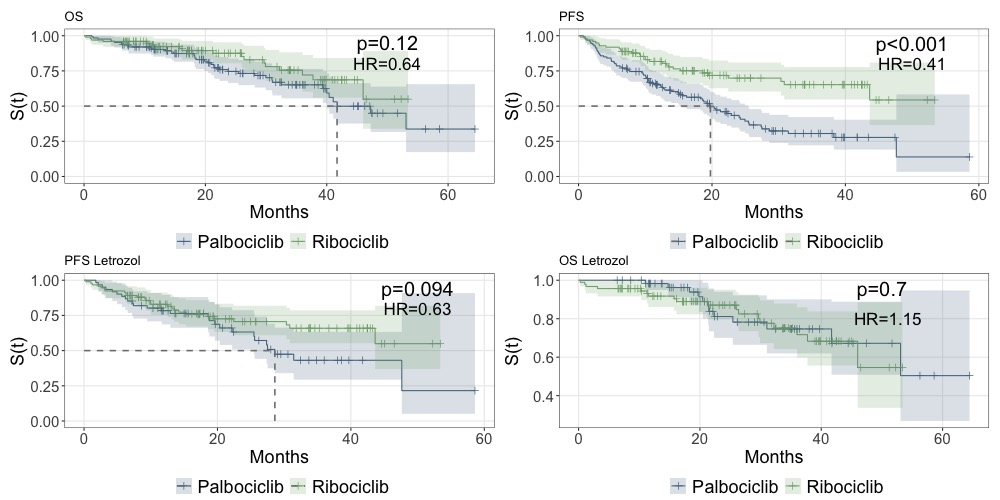
\includegraphics[scale=0.4]{figures/interest_curve_both.jpeg}%

\end{figure}


\begin{figure}[ht]
  \centering
  \caption{Cox Regression with palbociclib and Ribociclib - Progression Free Survival and Overall Survival}\label{fig:cox} 
  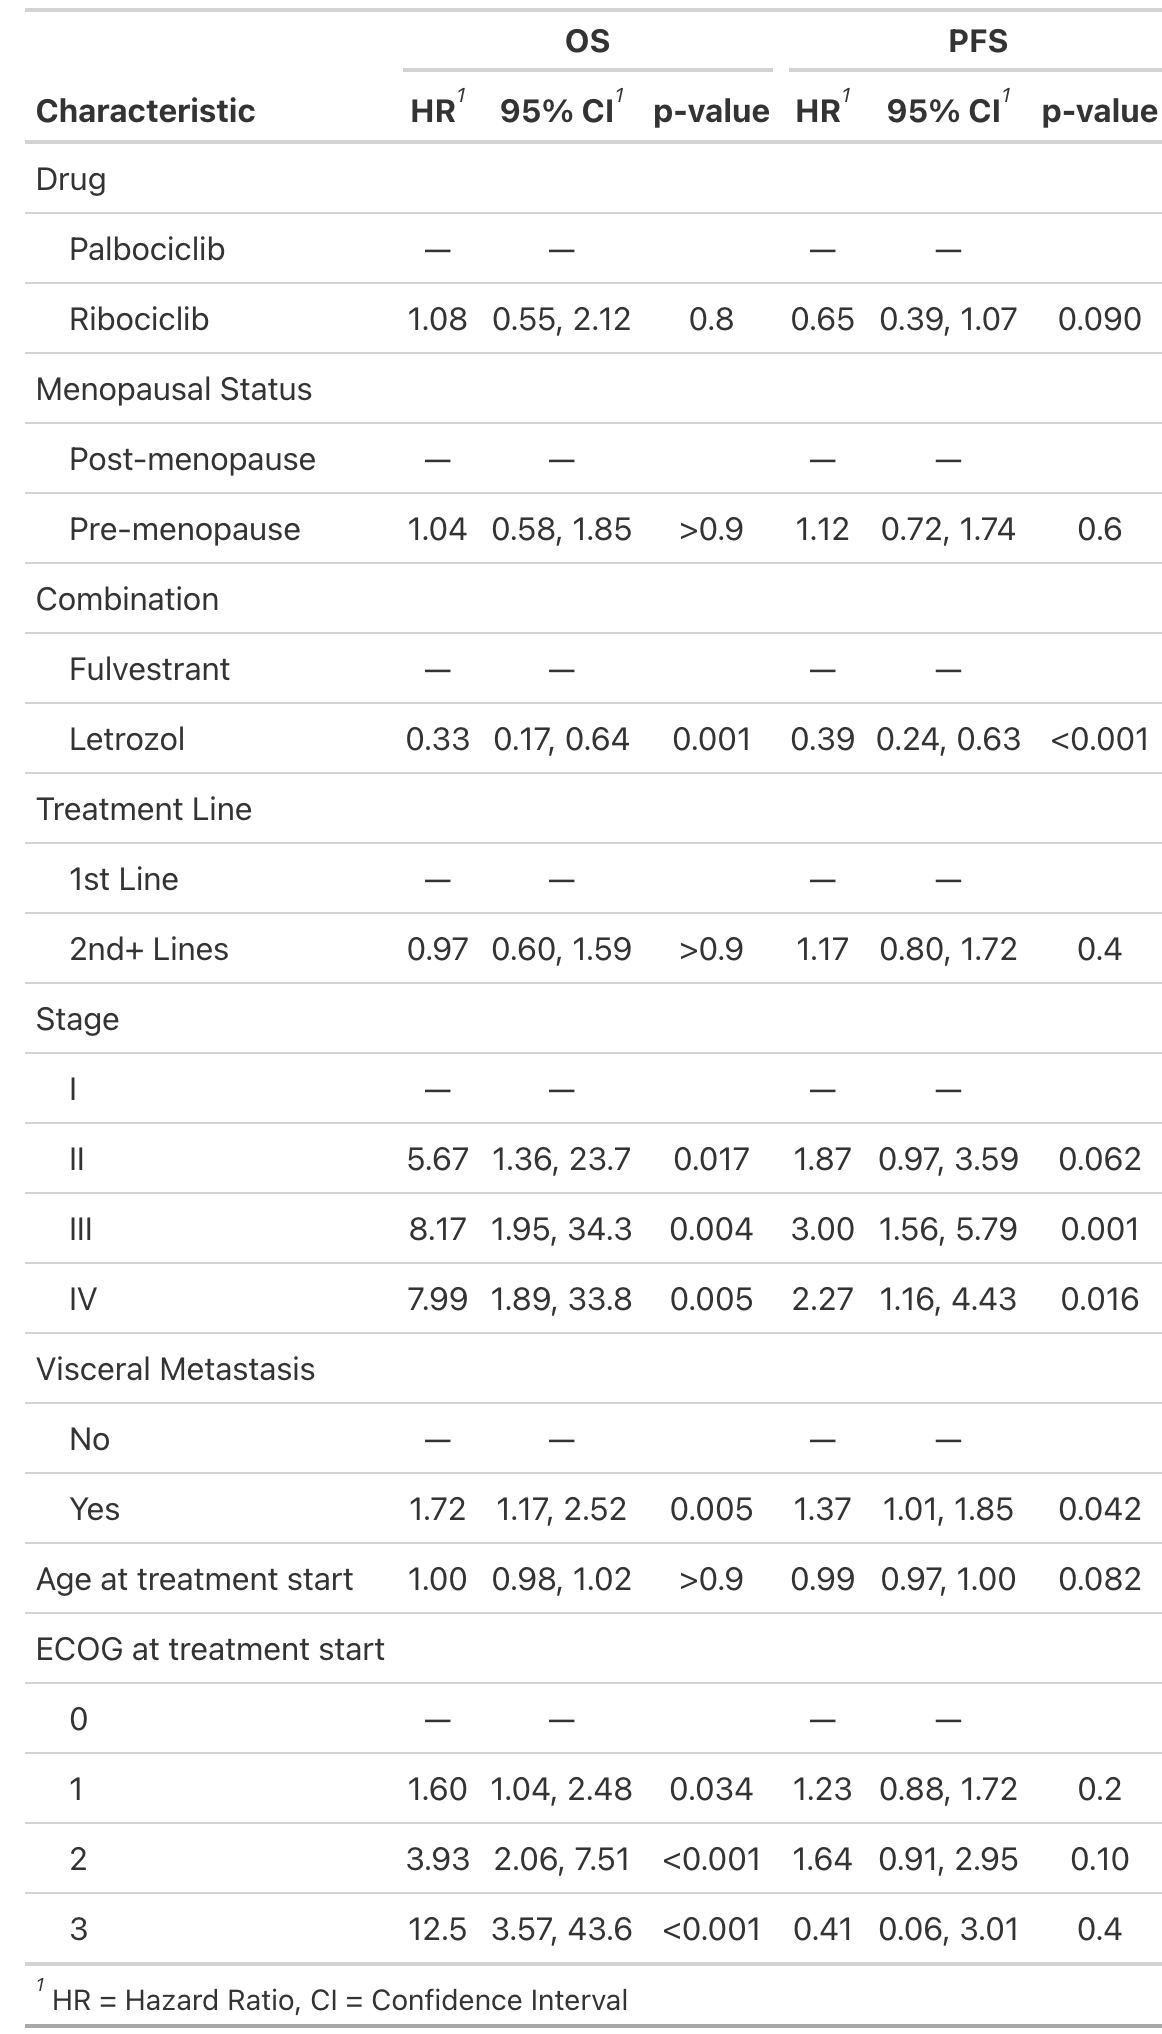
\includegraphics[scale=0.25]{figures/cox_both.png}%

\end{figure}

\begin{figure}[ht]
  \centering

  \caption{Comparision of traditional hormonotherapy and CDK4/6 inhibitors  }\label{fig:grouped} 
  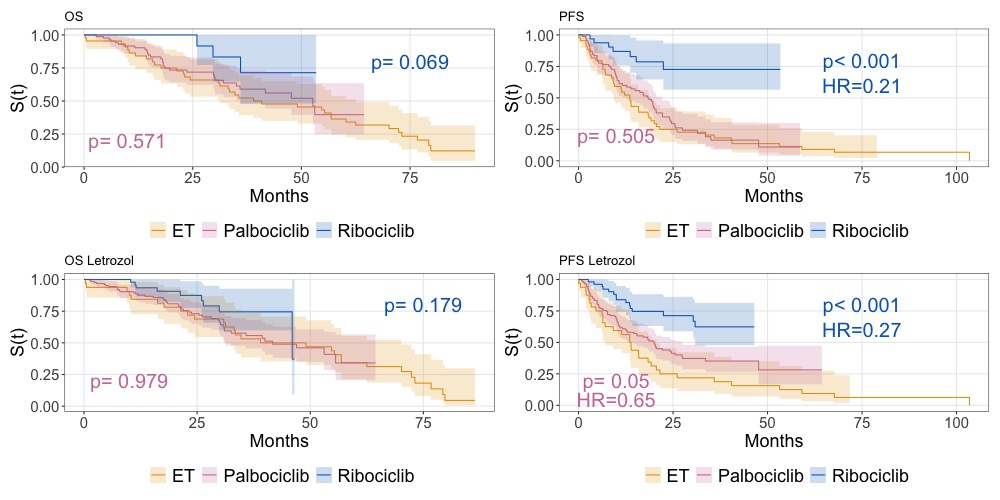
\includegraphics[scale=0.4]{figures/grouped_curve_both.jpeg}%

\end{figure}

\begin{figure}[ht]
  \centering

  \caption{Comparasion of palbociclib and ribociclib adjusted for propensity scores  }\label{fig:propensity} 
  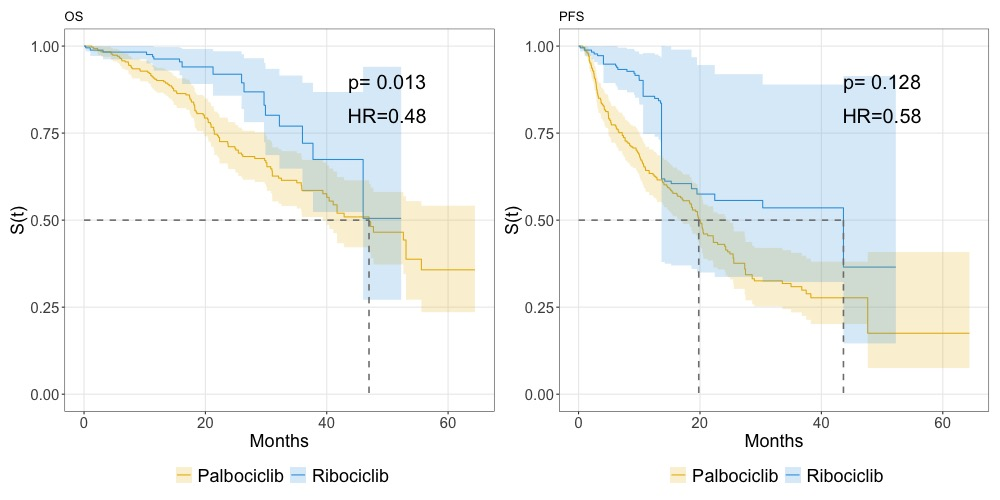
\includegraphics[scale=0.35]{figures/propensity_score_both.jpeg}%

\end{figure}
